\documentclass{article}
\usepackage{mathtools}
\usepackage[top=2in, bottom=1.5in, left=1in, right=1in]{geometry}
\usepackage{graphicx}
\usepackage[normalem]{ulem}
\usepackage{fancyhdr}
\usepackage{enumerate}
\pagestyle{fancyplain}

\lhead{PHYS 152 Section 10}

\rhead{A. Shawn Bandy 
(003635396)}


\begin{document}
\title{Lab \#5:  name}
\author{A. Shawn Bandy}
\date{March 13\textsuperscript{th}, 2013}
\maketitle
\begin{abstract}
Using resistors in parallel and in series with a DC power supply we measured voltage, current and resistance.  Using Ohm's Law we calculated these potentially unknown values
from our measurement.
\end{abstract}
\begingroup
	\section{Data and Data Tables}\hfill\\
		\let\clearpage\relax
			\subsection{DATA SHEET \#1}
	\begin{enumerate}[A.]
		\item	Circuit \#1: Direct measurements of resistors using handheld BK meter.  The uncertainties on these measurements are primarily from the instrument.  Assume an uncertainty of 0.1\%.\\
		
		$R_1 \pm \Delta R_1 = 29.77 \pm 0.0298 \Omega$\\
		$R_2 \pm \Delta R_2 = 50.04 \pm 0.0500 \Omega$\\
		
		\item Circuit \#1: Direct measurement of current I from power supply.  Assume an uncertainty of 1.0\% for the BK Ammeter values.
		
		$I_{POWER SUPPLY} \pm \Delta I = 0.11 \pm 0.0001 \Omega$\\
		
		$\Delta V_{READING\_POWER\_SUPPLY} = 8.6 V$\\
		
		These two numbers allow you to predict (via calculation using Ohm's Law) the equivalent resistance of whatever is attached to the power supply, imagining whatever is attached as a single resistor.  Make a prediction and do so now (ignore uncertainties):
		
		$R_{EQUIVALENT} = 78.18 \Omega$\\
		
		\item
			\begin{enumerate}[1.]
			
				\item Circuit \#1:  For each resistor, calculate potential changes (voltage) using Ohm's Law predicts for the potential change across each resistance.\\
				
				$\Delta V_{1CALC} \pm uncertainty = (I \pm \Delta I) \times [R_1 \pm \Delta R_1] = 5.5044 \pm  0.055 V$\\ 
				
				$\Delta V_{2CALC} \pm uncertainty = (I \pm \Delta I) \times [R_2 \pm \Delta R_2] = 3.2747 \pm 0.033 V$\\
			
				\item Show how you calculated the uncertainty on the first result above:
				
				$\sqrt{0.001^2 + 0.01^2} \times calculated  \Delta V_{1CALC} = 0.01005 * 5.5044 = 0.055$ \\
					
			\end{enumerate}
			
	\end{enumerate}
			\subsection{DATA SHEET \#2}
	\begin{enumerate}[A.]
		\item Circuit \#1: Direct measurement of potential changes (voltage) using the DMM across each resistor separately and both together.  Assume uncertainty of 0.05\%.\\
		
			$\Delta V_1 \pm uncertainty = 5.344 \pm 0.0027 V$\\
			$\Delta V_2 \pm uncertainty = 3.1904 \pm 0.0016 V$\\
			$\Delta V_{TOTAL} \pm uncertainty = 8.533 \pm 0.0043 V$\\
			
		\item Compare the values of voltages calculated in C1 (DATA SHEET \#1 with those directly measured in Part D above.  Do this by plotting the values appropriately on the grid below, setting the vertical scale so the uncertainty bars on the values are visible.  No horizontal axis scale is needed.  Simply plot the points next to each other.  For example, do the uncertainty ranges of $\Delta V_{1CALC} \pm uncertainty$ and $\Delta V_{1} \pm uncertainty$ overlap?\\
		
		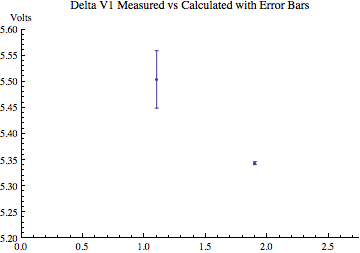
\includegraphics[width=200px]{lab6_graph1_deltav1}
		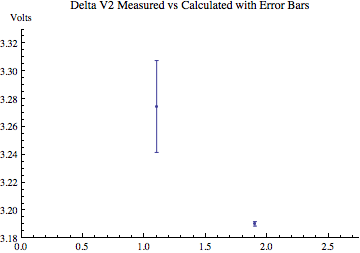
\includegraphics[width=200px]{lab6_graph2_deltav2}
		
		\item Comment on the above results.  Are the measurements consistent with each other? \\
		
		Within the given uncertainty terms, no they are not consistent with one another in the sense that the two sets of intervals do not overlap.  They do, however, appear to be correlated within a lower confidence interval.
\end{enumerate}
		
			\subsection{DATA TABLE \#3}
	\begin{enumerate}[A.]
		\item In circuit 1, is energy conserved around the loop of the circuit? \\
		\begin{enumerate}[1.]
			\item $[\Delta V_1 \pm uncertainty] + [\Delta V_2 \pm uncertainty] = 8.7791 \pm 0.088 V$ 
			
			\item Does the calculated [sum $\pm$ uncertainty] above overlap with the measured value $[\Delta V_1 \pm uncertainty]$?\\
			
			No, they do not overlap.  The gap between the uncertainty intervals is about 0.15 volts.\\
			
			If not, by what percentage does it differ?\\
			
			The differ by about \%1.0074.
			
			\item Based on your data, is energy conserved around the loop of the circuit?  State your reasoning below.\\
			
			Based on the data and given that the measurements were accurate and the given uncertainty intervals correct, then no I would not say energy is conserved around the loop of the circuit.  However, if this were a first experiment in this area then I would suggest that our data indicates that further experiments should be conducted by more controlled and rigorous methods.  I would also leave open the possibility that there is a physical explanation beyond measurement or calculation error as well.\\
			
		\end{enumerate}
	\end{enumerate}
	
					
			
			
			\subsection{DATA SHEET \#4}
	\begin{enumerate}[A.]
		\item Circuit \#2: Direct measurements of resistors in the range 500 $\Omega$ to 1200 $\Omega$ using handheld BK meter.  The uncertainties on these measurements are primarily from the instrument.  Assume an uncertainty of 0.1\% for the ohmmeter values. \\
		
			$R_1 \pm \Delta R_1 = 1010 \pm 0.101 \Omega $
			
			$R_2 \pm \Delta R_2 = 619 \pm 0.619 \Omega $
			
		\item Circuit \#2: Direct measurement of current $I$ and $I_1$ from power supply.  Assume an uncertainty of 1.0\% for the BK ammeter values.\\
		
			$I \pm \Delta I = 0.08 \pm 0.0008 A$ \\
			
			$V_{READING\_FROM\_POWER\_SUPPLY} = 25 V$ \\
			
			$R_{EQUIVALENT} = 312.5 \Omega$ \\
			
		\item Circuit \#2: Measured values: \\
			
			$I_1 \pm \Delta I_1 = 0.04 \pm 0.0004 A$ \\ 
			
			$I_2 \pm \Delta I_2 = 0.02 \pm 0.0002 A$ \\
			
			$\Delta V_1 \pm uncertainty = 25 \pm 1.25 V$\\
			
		\item For each resistor, calculate potential changes (voltage) using Ohm's Law.  You have the resistor values and the current through each one.  Calculate what Ohm's Law predicts for the potential change across each resistance. \\
		
			$\Delta V_{1CALC} \pm uncertainty = (I_1 \pm \Delta I_1) \times [R_1 \pm \Delta R_1] =  40.4 \pm 0.406 V$\\ 
			
			$\Delta V_{2CALC} \pm uncertainty = (I_2 \pm \Delta I_2) \times [R_2 \pm \Delta R_2] =  12.38 \pm 0.124 V$\\ 
\end{enumerate}			
			\subsection{DATA SHEET \#5}
	\begin{enumerate}[A.]
		\item Show how you calculated the uncertainty on the first result above.\\ 
		
		$\sqrt{0.01^2 + 0.001^2} * \Delta V_{1CALC}$\\
		
		\item $(I_1 \pm \Delta I_1) + (I_2 \pm \Delta I_2) = 0.02 + 0.04 = 0.06 \pm 0.0006 A$ \\
		
		\item Does the sum above equal the measured $I \pm \Delta I$ from the power supply?  Show these two values with their uncertainty ranges on the graph to the right and comment on your results. \\ 
		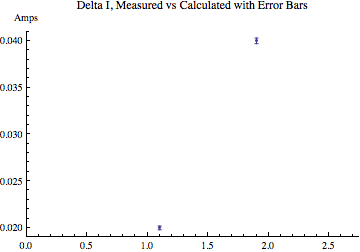
\includegraphics[width=200px]{lab6_graph3_cur2errorbars}
		
	\end{enumerate}
			\subsection{DATA SHEET \#6}
	\begin{enumerate}[A.]
		\item In circuit 2, is energy conserved around the various closed loops of the circuit?  There are three possible closed loops in this circuit, shown in the diagram (omitted from this report) as dashed lines simply labeled as 1, 2, 3.  Show explicitly, for each of these loops, using the appropriate symbols in one line and the same equation in the second line that the sum of the potential differences around each loop is zero.  If your sums are not zero, state why you think they do not.\\ 
		
	Loop 3: $0 + I_1 * R_1 + 0 =  40.4 V$\\
	Loop 2: $0 + I_2 * R_2 + 0 = 12.35 V$\\
	Loop1: $Measured current * Equivalent Resistor = 25V$\\
	
	Sum of loops 40.4 - 12.35 - 25 = 3.05\\
	
	The sum of our loops does not equal 0 which suggests either there was an error in how we carried out the procedure or in our measurements or there is a an actual physical phenomenon that was not controlled for in this experiment.
	
	\end{enumerate}
\endgroup
\begingroup
	\section{Graphs}\hfill\\
		See Data Tables section
\endgroup
\begingroup
	\section{Uncertainty Calculations}\hfill\\
		\let\clearpage\relax
			See Data Tables section
\endgroup
\begingroup
	\section{Results}\hfill\\
		\let\clearpage\relax
			See Data Tables section
\endgroup
\begingroup
	\section{Discussion}\hfill\\
		\let\clearpage\relax
			In this lab we measured the electrical properties of two circuits.  The first circuit contained a DC power supply and two resistors in series.  We measured the voltage across each resistor as well as the current between the power supply and each resistor.  The second circuit contained  a DC power supply and two resistors in series.  We measured current and used the known values of the resistors to calculate the voltage in the nested circuit loops.  The objective for testing each circuit was to demonstrate the conservation of energy in electrical circuits by comparing measurements and estimations.  In the case of the both circuits, we could not demonstrate the conservation of energy although the data would warrant further investigation and experimentation.  

Although the uncertainty factors were given for the equipment I do not suspect that our equipment was faulty and so our data probably cannot be explained by this kind of error.  It is possible that that environmental electrical and magnetic fields interfered with the circuitry.  Again, given the size of our errors I suspect this would only account for some of the variance in our data.  There was an unusual amount of confusion about the procedure for Circuit \#2 which is a likely source of error.
\endgroup
\begingroup
	\section{Answers }\hfill\\
		\let\clearpage\relax
			All questions for this lab were on the Data Tables worksheets and so are in-line in this document as well.
\endgroup
\end{document}